\documentclass[ignorenonframetext,8pt,aspectratio=169]{beamer}

\usepackage{umut}
\usepackage{umuttr}
\usepackage{usynsem}
\usepackage[utf8]{inputenc}
\usepackage{uling}
\usepackage{natbib,unatbib}
\usepackage{linguex}
         \renewcommand{\refdash}{}
\usepackage{ubeamer}
\usepackage{verbatim}
\usepackage{adjustbox}
\usepackage{fancyvrb}

\usepackage{tikz-qtree}
\usetikzlibrary{er,positioning}

\title{Wh-movement}
\author{\  \\  {\it Partly based on Koeneman \& Zeiljstra (2017)} \\ \vspace{20pt} Umut \"Ozge\\  }

\date{COGS 532: Theoretical Linguistics\\ METU, Informatics}

\begin{document}

\begin{frame}\frametitle{}
\thispagestyle{empty}
\maketitle
\end{frame}

\begin{frame}[t,plain]{Where to land?}

\ex. Which chair has Adrian always liked?

\ex. Adrian has always liked this yellow chair.

\bigskip
\bigskip
\bigskip
\bigskip

\begin{center}
\Tree[.{FinP} [.{DP} Adrian ] [.{Fin'} [.{Fin} has ] [.{VP} \edge[roof]; {always liked this yellow chair} ] ] ] 
\end{center}


\end{frame}

\begin{frame}[t,plain]{Head versus phrase positions}
\bigskip

\Tree[.{S} [.{Y} \edge[roof]; \colb{Which chair} ] [.{K} [.{X} \colr{has} ] [.{FinP} [.{DP} Adrian ] [.{Fin'} [.{Fin} \colr{<has>} ] [.{VP} \edge[roof]; {always liked \colb{<this yellow chair>}} ] ] ] ] ] 
\end{frame}

\begin{frame}[t,plain]{Head versus phrase positions}

\bigskip

\begin{center}
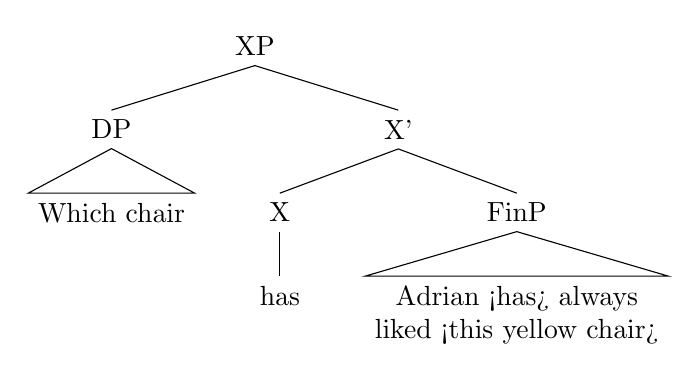
\begin{tikzpicture}
\tikzset{level distance=30pt, sibling distance=20pt}
\tikzset{every tree node/.style={align=center,anchor=north}}
\Tree[.{XP} [.{DP} \edge[roof]; {Which chair} ] [.{X'} [.{X} has ] [.{FinP} \edge[roof]; {Adrian <has> always\\liked <this yellow chair>} ] ] ]
\end{tikzpicture}
\end{center}

\end{frame}

\begin{frame}[t,plain]{A head position commanding FinP}

\bigskip

\ex. \a. I think that Adrian has always liked this yellow chair.
\b.  I asked if Adrian has always liked this yellow chair.

\begin{center}
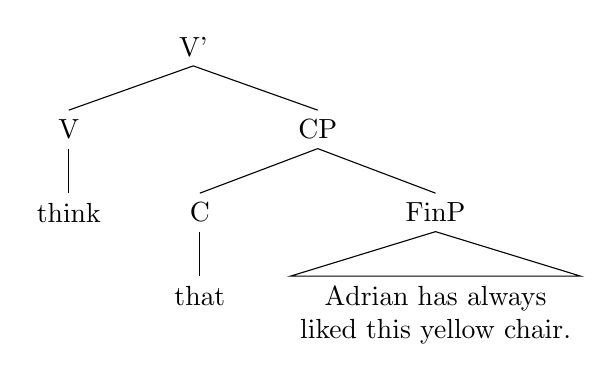
\begin{tikzpicture}
\tikzset{level distance=30pt, sibling distance=20pt}
\tikzset{every tree node/.style={align=center,anchor=north}}
		\Tree[.{V'} [.{V} think ] [.{CP} [.{C} that ] [.{FinP} \edge[roof]; {Adrian has always\\liked this yellow chair.} ] ] ] 
\end{tikzpicture}
\hspace{10pt}
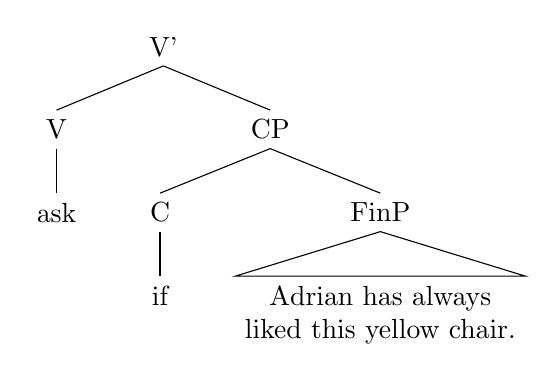
\begin{tikzpicture}
\tikzset{level distance=30pt, sibling distance=20pt}
\tikzset{every tree node/.style={align=center,anchor=north}}
		\Tree[.{V'} [.{V} ask ] [.{CP} [.{C} if ] [.{FinP} \edge[roof]; {Adrian has always\\liked this yellow chair.} ] ] ] 
\end{tikzpicture}
\end{center}
\end{frame}

\begin{frame}[t,plain]{A head position commanding FinP}

\bigskip

\ex. \a. I think that Adrian has always liked this yellow chair.
\b.  I asked if Adrian has always liked this yellow chair.

\begin{center}
\begin{tikzpicture}
\tikzset{level distance=30pt, sibling distance=18pt}
\tikzset{every tree node/.style={align=center,anchor=north}}
		\Tree[.{V'} [.{V} think ] [.{CP} [.{C} that\\\setavm{\[cat  & c \\ embed.  & + \\ type  & decl.\]} ] [.{FinP} \edge[roof]; {Adrian has always\\liked this yellow chair.} ] ] ] 
\end{tikzpicture}
\begin{tikzpicture}
\tikzset{level distance=30pt, sibling distance=18pt}
\tikzset{every tree node/.style={align=center,anchor=north}}
\Tree[.{V'} [.{V} ask ] [.{CP} [.{C} if\\\setavm{\[cat  & c \\ embed.  & + \\ type  & ques.\]}
 ] [.{FinP} \edge[roof]; {Adrian has always\\liked this yellow chair.} ] ] ] 
\end{tikzpicture}
\end{center}
\end{frame}

\begin{frame}[t,plain]{}


\begin{center}
\begin{tikzpicture}
\tikzset{level distance=30pt, sibling distance=20pt}
\tikzset{every tree node/.style={align=center,anchor=north}}
\Tree[.{CP} [.{DP} \edge[roof]; {Which chair} ] [.{C'} [.{C} has\\\setavm{\[cat  & c \\ embed.  & - \\ type  & ques.\]} ] [.{FinP} \edge[roof]; {Adrian <has> always\\liked <this yellow chair>} ] ] ]
\end{tikzpicture}
\end{center}
\end{frame}

\begin{frame}[t,plain]{Simple yes/no questions}

\ex. Has Adrian always liked this chair?

\begin{center}
\begin{tikzpicture}
\tikzset{level distance=30pt, sibling distance=20pt}
\tikzset{every tree node/.style={align=center,anchor=north}}
\Tree[.{CP} [.{C} has\\\setavm{\[cat  & c \\ embed.  & - \\ type  & ques.\]} ] [.{FinP} \edge[roof]; {Adrian <has> always\\liked this yellow chair} ] ] 
\end{tikzpicture}
\end{center}

\end{frame}

\begin{frame}[t,plain]{Deriving a question}

\ex. Has Adrian always liked this chair?

\begin{center}
\begin{tikzpicture}
\tikzset{level distance=30pt, sibling distance=20pt}
\tikzset{every tree node/.style={align=center,anchor=north}}
\Tree[.{CP} [.{C\\\setavm{\[cat  & c \\ embed.  & - \\ type  & ques.\]}}  ] [.{FinP} [.{DP} Adrian ] [.{Fin'} [.{Fin} has ] [.{VP} {always liked this yellow chair} ] ] ] ] 
\end{tikzpicture}
\end{center}

\end{frame}

\begin{frame}[t,plain]{Some predictions}

\ex. \a. *I wonder has Adrian always liked this chair?
\b. *I wonder which yellow chair has Adrian always liked?

\end{frame}

\begin{frame}[t,plain]{Wh-phrase landing site}

\bigskip
\bigskip
\bigskip
\bigskip
\bigskip

{\small
\begin{center}
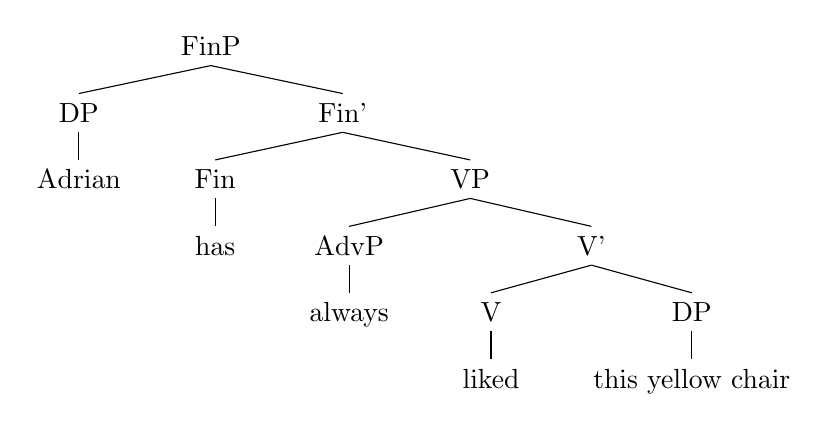
\begin{tikzpicture}
\tikzset{level distance=24pt, sibling distance=20pt}
\tikzset{every tree node/.style={align=center,anchor=north}}
\Tree[.{FinP} [.{DP} Adrian ] [.{Fin'} [.{Fin} has ] [.{VP} [.{AdvP} always ] [.{V'} [.{V} liked ] [.{DP} {this yellow chair} ] ] ] ] ] 
\end{tikzpicture}
\end{center}
		}
\end{frame}
\begin{frame}[t,plain]{Wh-phrase landing site}

\bigskip

{\small
\begin{center}
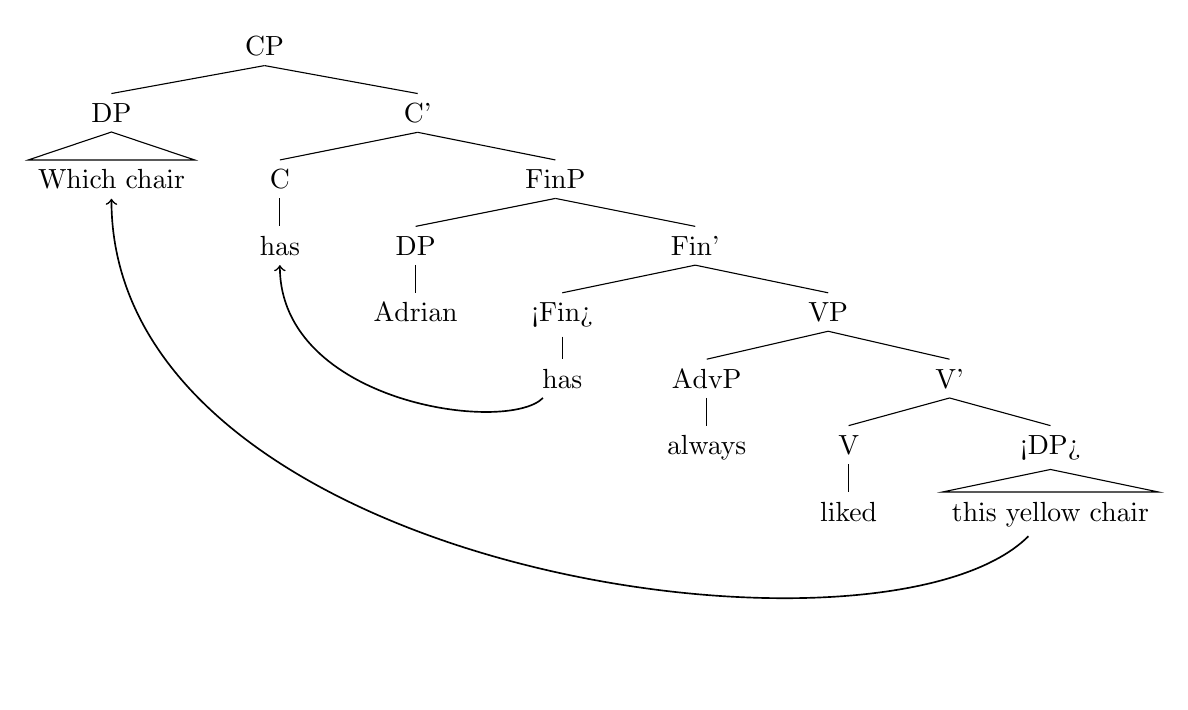
\begin{tikzpicture}
\tikzset{level distance=24pt, sibling distance=20pt}
\tikzset{every tree node/.style={align=center,anchor=north}}
		\Tree[.{CP} [.{DP} \edge[roof]; \node(wh){Which chair}; ] [.{C'} [.{C} \node(c){has}; ] [.{FinP} [.{DP} Adrian ] [.{Fin'} [.{<Fin>} \node(fin){has}; ] [.{VP} [.{AdvP} always ] [.{V'} [.{V} liked ] [.{<DP>} \edge[roof]; \node(base){this yellow chair}; ] ] ] ] ] ] ] 
\draw[semithick,->] (base)..controls +(south west:3) and +(south:5)..(wh);
\draw[semithick,->] (fin)..controls +(south west:1) and +(south:2)..(c);
\end{tikzpicture}
\end{center}
		}
\end{frame}








\begin{frame}[t,plain]{Some open questions}

\ex. \a. I wonder which yellow chair Adrian has always liked?
\b. *I wonder which yellow chair if Adrian has always liked?

\end{frame}
\end{document}

